\documentclass[12pt,a4paper]{article}
\usepackage[top=16mm,bottom=18mm,left=16mm,right=16mm,headheight=0pt,headsep=0mm,footskip=10mm]{geometry}
\usepackage{iftex}
\ifPDFTeX
  \usepackage[utf8]{inputenc}
  \usepackage[T5]{fontenc}
  \usepackage{mathptmx}
\else
  \usepackage{fontspec}
  \usepackage{mathptmx}
  \setmainfont{Times New Roman}
\fi
\usepackage{amsmath,amssymb}
\usepackage{xcolor}
\usepackage{tikz}
\usepackage{graphicx}
\usepackage{array,tabularx}
\usepackage{enumitem}
\usepackage{fancyhdr}
\usepackage{lastpage}

\definecolor{questionpurple}{RGB}{137,38,143}
\definecolor{answerblue}{RGB}{35,45,140}

\setlength{\parindent}{0pt}
\setlength{\parskip}{0pt}
\renewcommand{\baselinestretch}{1.12}
\pagestyle{fancy}
\fancyhf{}
\renewcommand{\headrulewidth}{0pt}
\fancyfoot[L]{\small Chuyên đề I -- Toán 11}
\fancyfoot[R]{\small Trang \thepage/\pageref{LastPage} -- Đề test số 01}
\renewcommand{\footrulewidth}{.4pt}

\newlist{questions}{enumerate}{1}
\setlist[questions]{label=\textcolor{questionpurple}{\bfseries Câu \arabic*.},leftmargin=0pt,itemindent=16mm,labelwidth=14mm,labelsep=2mm,align=left,itemsep=9pt,topsep=7pt,parsep=0pt}
\newcommand{\answerlabel}[1]{\tikz[baseline=(choice.base)]\node[draw=black!65,text=answerblue,circle,inner sep=0pt,minimum size=4.8mm,line width=.4pt,font=\normalsize] (choice) {#1};}
\newcommand{\fourchoices}[4]{\par\begingroup\setlength{\tabcolsep}{0pt}\renewcommand{\arraystretch}{1.35}\begin{tabularx}{\linewidth}{@{}*{4}{>{\raggedright\arraybackslash}X}@{}}\answerlabel{A}~#1 & \answerlabel{B}~#2 & \answerlabel{C}~#3 & \answerlabel{D}~#4\end{tabularx}\endgroup}
\newcommand{\twochoices}[4]{\par\begingroup\setlength{\tabcolsep}{0pt}\renewcommand{\arraystretch}{1.5}\begin{tabularx}{\linewidth}{@{}*{2}{>{\raggedright\arraybackslash}X}@{}}\answerlabel{A}~#1 & \answerlabel{B}~#2 \\ \answerlabel{C}~#3 & \answerlabel{D}~#4\end{tabularx}\endgroup}

\begin{document}

\noindent
\begin{minipage}[t]{.35\textwidth}
  \centering
  {\bfseries CHUYÊN ĐỀ I -- TOÁN -- 11\par}
  \vspace{2pt}
  \rule{.72\linewidth}{.4pt}\par
  \vspace{3pt}
  CHƯƠNG I\par
  \vspace{4pt}
  {\itshape ĐỀ TEST SỐ 01\par}
\end{minipage}\hfill
\begin{minipage}[t]{.62\textwidth}
  \centering
  {\bfseries HÀM SỐ LƯỢNG GIÁC\par
  VÀ PHƯƠNG TRÌNH LƯỢNG GIÁC\par}
  \vspace{5pt}
  {\small\bfseries BÀI 3. HÀM SỐ LƯỢNG GIÁC\par}
\end{minipage}

\vspace{7mm}
\noindent
\begin{minipage}[t]{.72\textwidth}
  \textbf{Họ, tên thí sinh:}\dotfill\par
  \vspace{3pt}
  \textbf{Số báo danh:}\dotfill
\end{minipage}\hfill
\begin{minipage}[t]{.25\textwidth}
  \raggedleft
  \setlength{\fboxsep}{4pt}
  \fbox{\textbf{Đề test số: 01}}
\end{minipage}

\vspace{5mm}
\textbf{PHẦN I. Câu trắc nghiệm nhiều phương án lựa chọn.} Thí sinh trả lời từ câu 1 đến câu 12. Mỗi câu hỏi thí sinh chỉ chọn một phương án.

\begin{questions}
  \item Khẳng định nào sau đây là sai?
  \twochoices
    {Hàm số $y=\tan x$ có tập giá trị là $\mathbb{R}$.}
    {Hàm số $y=\cos x$ có tập giá trị là $[-1;1]$.}
    {Hàm số $y=\sin x$ có tập giá trị là $[-1;1]$.}
    {Hàm số $y=\cot x$ có tập giá trị là $[0;\pi]$.}

  \item Tập xác định của hàm số $y=\cot x$ là
  \twochoices
    {$D=\mathbb{R}$.}
    {$D=\mathbb{R}\setminus\left\{\left.k\dfrac{\pi}{2}\,\right|\,k\in\mathbb{Z}\right\}$.}
    {$D=\mathbb{R}\setminus\left\{\left.\pi+k\dfrac{\pi}{2}\,\right|\,k\in\mathbb{Z}\right\}$.}
    {$D=\mathbb{R}\setminus\left\{\left.k\pi\,\right|\,k\in\mathbb{Z}\right\}$.}

  \item Tập xác định của hàm số $y=\tan\left(3x+\dfrac{\pi}{4}\right)$ là
  \twochoices
    {$D=\mathbb{R}\setminus\left\{\left.\dfrac{\pi}{12}+k\pi\,\right|\,k\in\mathbb{Z}\right\}$.}
    {$D=\mathbb{R}\setminus\left\{\left.k\pi\,\right|\,k\in\mathbb{Z}\right\}$.}
    {$D=\mathbb{R}$.}
    {$D=\mathbb{R}\setminus\left\{\left.\dfrac{\pi}{12}+\dfrac{k\pi}{3}\,\right|\,k\in\mathbb{Z}\right\}$.}

  \item Trong các hàm số sau, hàm số nào là hàm số lẻ?
  \fourchoices{$y=\sin x$.}{$y=\sin x+\cos x$.}{$y=-\cos x$.}{$y=\cos x$.}

  \item Trong các hàm số sau, hàm số nào là hàm số chẵn?
  \fourchoices{$y=\cos 3x$.}{$y=-\sin x$.}{$y=\sin 3x$.}{$y=\sin 2x+\cos 2x$.}

  \item Tìm tập giá trị $T$ của hàm số $y=2\cos x+3$.
  \fourchoices{$T=[1;5]$.}{$T=[-1;1]$.}{$T=\mathbb{R}$.}{$T=[0;3]$.}

  \item Giá trị nhỏ nhất và giá trị lớn nhất của hàm số $y=3\sin 2x-5$ lần lượt là:
  \fourchoices{$-8$ và $-2$.}{$2$ và $8$.}{$-5$ và $2$.}{$-5$ và $3$.}

  \item Gọi $M,m$ lần lượt là giá trị lớn nhất và giá trị nhỏ nhất của hàm số $y=2\cos\left(x+\dfrac{\pi}{3}\right)$. Tính $P=M-m$.
  \fourchoices{$P=2\sqrt2$.}{$P=4$.}{$P=\sqrt2$.}{$P=2$.}

  \item Hàm số $y=\tan x$ đồng biến trên khoảng nào trong các khoảng sau?
  \fourchoices{$(0;\pi)$.}{$(\pi;2\pi)$.}{$\left(-\dfrac{\pi}{2};\pi\right)$.}{$\left(\dfrac{3\pi}{2};\dfrac{5\pi}{2}\right)$.}
\end{questions}

\newpage

\begin{center}
  {\small\bfseries\itshape CHUYÊN ĐỀ I -- TOÁN -- 11 -- HÀM SỐ LƯỢNG GIÁC VÀ PHƯƠNG TRÌNH LƯỢNG GIÁC}
\end{center}

\begin{questions}[resume,itemsep=7pt,topsep=3pt]
  \item Hàm số nào có đồ thị như hình dưới đây?
  \begin{center}
  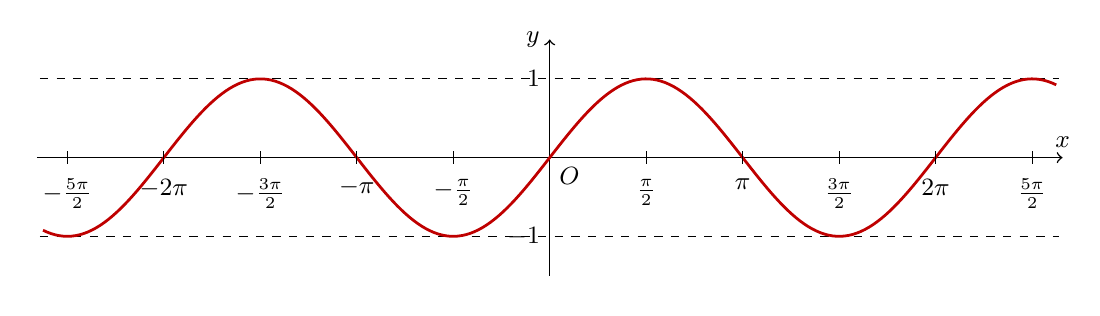
\begin{tikzpicture}[x=.78cm,y=1.0cm,font=\small]
    \clip (-8.5,-1.65) rectangle (8.5,1.65);
    \draw[->,line width=.55pt] (-8.35,0) -- (8.35,0) node[above] {$x$};
    \draw[->,line width=.55pt] (0,-1.5) -- (0,1.5) node[left] {$y$};
    \draw[dashed,line width=.4pt] (-8.3,1) -- (8.3,1);
    \draw[dashed,line width=.4pt] (-8.3,-1) -- (8.3,-1);
    \draw[red!75!black,line width=1pt,samples=250,domain=-8.25:8.25] plot(\x,{sin(\x r)});
    \foreach \x/\lab in {-7.854/{-\frac{5\pi}{2}},-6.283/{-2\pi},-4.712/{-\frac{3\pi}{2}},-3.142/{-\pi},-1.571/{-\frac{\pi}{2}},1.571/{\frac{\pi}{2}},3.142/{\pi},4.712/{\frac{3\pi}{2}},6.283/{2\pi},7.854/{\frac{5\pi}{2}}}{
      \draw (\x,.08)--(\x,-.08) node[below=2pt] {$\lab$};
    }
    \node[left] at (0,1) {$1$};
    \node[left] at (0,-1) {$-1$};
    \node[below right] at (0,0) {$O$};
  \end{tikzpicture}
  \end{center}
  \fourchoices{$y=\sin x$.}{$y=2\sin x$.}{$y=\cos x$.}{$y=\sin 2x$.}

  \item Đường cong hình bên dưới là đồ thị của hàm số nào trong bốn hàm số sau?
  \begin{center}
  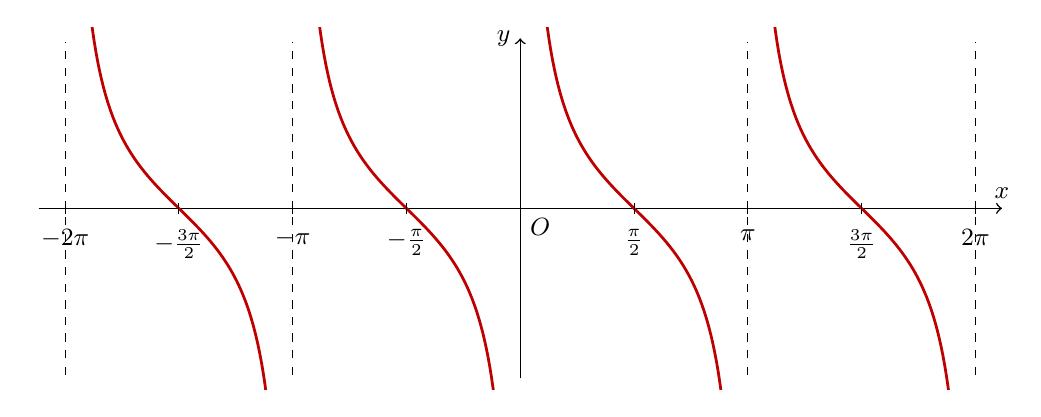
\begin{tikzpicture}[x=.92cm,y=.9cm,font=\small]
    \clip (-6.8,-2.55) rectangle (6.8,2.55);
    \draw[->,line width=.55pt] (-6.65,0) -- (6.65,0) node[above] {$x$};
    \draw[->,line width=.55pt] (0,-2.4) -- (0,2.4) node[left] {$y$};
    \foreach \x in {-6.283,-3.142,0,3.142,6.283}{
      \draw[dashed,line width=.4pt] (\x,-2.35)--(\x,2.35);
    }
    \draw[red!75!black,line width=1pt,samples=120,domain=-6.18:-3.25] plot(\x,{1/tan(\x r)});
    \draw[red!75!black,line width=1pt,samples=120,domain=-3.03:-.10] plot(\x,{1/tan(\x r)});
    \draw[red!75!black,line width=1pt,samples=120,domain=.10:3.03] plot(\x,{1/tan(\x r)});
    \draw[red!75!black,line width=1pt,samples=120,domain=3.25:6.18] plot(\x,{1/tan(\x r)});
    \foreach \x/\lab in {-6.283/{-2\pi},-4.712/{-\frac{3\pi}{2}},-3.142/{-\pi},-1.571/{-\frac{\pi}{2}},1.571/{\frac{\pi}{2}},3.142/{\pi},4.712/{\frac{3\pi}{2}},6.283/{2\pi}}{
      \draw (\x,.08)--(\x,-.08) node[below=2pt] {$\lab$};
    }
    \node[below right] at (0,0) {$O$};
  \end{tikzpicture}
  \end{center}
  \fourchoices{$y=\sin x$.}{$y=\cos x$.}{$y=\cot x$.}{$y=\tan x$.}

  \item Cho hàm số $y=\sin x$ có đồ thị như hình vẽ dưới đây.
  \begin{center}
  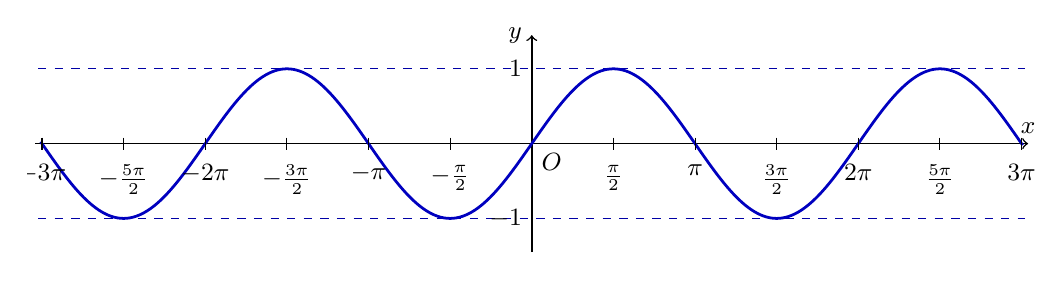
\begin{tikzpicture}[x=.66cm,y=.95cm,font=\small]
    \clip (-9.7,-1.55) rectangle (9.7,1.55);
    \draw[->,line width=.55pt] (-9.55,0) -- (9.55,0) node[above] {$x$};
    \draw[->,line width=.55pt] (0,-1.45) -- (0,1.45) node[left] {$y$};
    \draw[blue!65!black,dashed,line width=.45pt] (-9.5,1)--(9.5,1);
    \draw[blue!65!black,dashed,line width=.45pt] (-9.5,-1)--(9.5,-1);
    \draw[blue!75!black,line width=1pt,samples=320,domain=-9.45:9.45] plot(\x,{sin(\x r)});
    \foreach \x/\lab in {-9.425/{-3\pi},-7.854/{-\frac{5\pi}{2}},-6.283/{-2\pi},-4.712/{-\frac{3\pi}{2}},-3.142/{-\pi},-1.571/{-\frac{\pi}{2}},1.571/{\frac{\pi}{2}},3.142/{\pi},4.712/{\frac{3\pi}{2}},6.283/{2\pi},7.854/{\frac{5\pi}{2}},9.425/{3\pi}}{
      \draw (\x,.08)--(\x,-.08) node[below=2pt] {$\lab$};
    }
    \node[left] at (0,1) {$1$};
    \node[left] at (0,-1) {$-1$};
    \node[below right] at (0,0) {$O$};
  \end{tikzpicture}
  \end{center}
  Dựa vào đồ thị, hãy cho biết có bao nhiêu giá trị của $x$ trên đoạn $[-3\pi;3\pi]$ để $\sin x=0$?
  \fourchoices{$5$.}{$7$.}{$11$.}{$13$.}
\end{questions}

\vspace{3mm}
\textbf{PHẦN II. Câu trắc nghiệm đúng sai.} Thí sinh trả lời từ câu 1 đến câu 4. Trong mỗi ý a), b), c), d) ở mỗi câu, thí sinh chọn đúng hoặc sai.

\begin{questions}[start=1,itemsep=6pt,topsep=4pt]
  \item Cho biểu thức $F=\cos^2 a+2\sin a+2$.
  \begin{enumerate}[label=\alph*),leftmargin=7mm,labelsep=1mm,itemsep=3pt,topsep=3pt,parsep=0pt]
    \item Với $a=\dfrac{\pi}{2}$ thì $F=4$.
    \item $F=\sin^2 a+2\sin a+3$.
    \item $F$ đạt giá trị lớn nhất $\Leftrightarrow \cos a=1$.
    \item Giá trị nhỏ nhất của $F$ là $0$.
  \end{enumerate}

  \item Cho biểu thức $A=2\sin x-1$.
  \begin{enumerate}[label=\alph*),leftmargin=7mm,labelsep=1mm,itemsep=3pt,topsep=3pt,parsep=0pt]
    \item $\max A=3$.
    \item $A$ đạt GTNN tại $x=\dfrac{3\pi}{2}$.
    \item $\max A+\min A=-2$.
    \item Có $8$ giá trị nguyên của $m\in[-10;10]$ sao cho $m\le A,\ \forall x\in\mathbb{R}$.
  \end{enumerate}
\end{questions}

\newpage

\begin{center}
  {\small\bfseries\itshape CHUYÊN ĐỀ I -- TOÁN -- 11 -- HÀM SỐ LƯỢNG GIÁC VÀ PHƯƠNG TRÌNH LƯỢNG GIÁC}
\end{center}

\begin{questions}[resume,itemsep=6pt,topsep=3pt]
  \item Cho biểu thức $y=f(x)=\sin^6x+\cos^6x$. Các mệnh đề sau đúng hay sai?
  \begin{enumerate}[label=\alph*),leftmargin=7mm,labelsep=1mm,itemsep=3pt,topsep=3pt,parsep=0pt]
    \item $f(x)$ xác định trên $\mathbb{R}$.
    \item $f(x)=1-\dfrac{3}{4}\sin^2 2x$.
    \item Không tồn tại $x\in\mathbb{R}$ để $f(x)=0$.
    \item Giá trị lớn nhất của biểu thức $f(x)$ bằng $2$.
  \end{enumerate}

  \item Số giờ có ánh sáng của một thành phố $A$ trong ngày thứ $t$ của năm 2023 được cho bởi hàm số
  \[
    y=4\sin\left[\dfrac{\pi}{178}(t-60)\right]+10,
    \qquad t\in\mathbb{Z}\ \text{và}\ 0<t\le365.
  \]
  \begin{enumerate}[label=\alph*),leftmargin=7mm,labelsep=1mm,itemsep=3pt,topsep=3pt,parsep=0pt]
    \item Trong ngày thứ $60$, số giờ có ánh sáng của thành phố $A$ là $10$.
    \item Số giờ có ánh sáng trong một ngày của thành phố $A$ luôn lớn hơn hoặc bằng $6$.
    \item Số giờ có ánh sáng trong một ngày của thành phố $A$ nhiều nhất bằng $10$.
    \item Ngày 29 tháng 5 năm 2023, thành phố $A$ có nhiều giờ ánh sáng mặt trời nhất.
  \end{enumerate}
\end{questions}

\vspace{3mm}
\textbf{PHẦN III. Câu trắc nghiệm trả lời ngắn.} Thí sinh trả lời từ câu 1 đến câu 6.

\begin{questions}[start=1,itemsep=8pt,topsep=5pt]
  \item Tập giá trị của hàm số $y=5+4\sin 2x\cos 2x$ chứa tất cả bao nhiêu giá trị nguyên?

  \item Giả sử khi một con sóng biển đi qua một cái cọc ở ngoài khơi, chiều cao của nước được mô hình hoá bởi hàm số
  \[
    h(t)=90\cos\left(\dfrac{\pi}{10}t\right),
  \]
  trong đó $h(t)$ là độ cao tính bằng centimet trên mực nước biển trung bình tại thời điểm $t$ giây. Tìm chiều cao của sóng, tức là khoảng cách theo phương thẳng đứng giữa đáy và đỉnh của sóng.

  \item Gọi $M$ và $m$ lần lượt là giá trị lớn nhất và giá trị nhỏ nhất của hàm số $y=\cos 2x+\cos x$. Tính tổng $M+m$. (kết quả làm tròn đến hàng phần trăm)

  \item Số giờ có ánh sáng của một thành phố $X$ ở vĩ độ $40^\circ$ Bắc trong ngày thứ $t$ của một năm không nhuận được cho bởi hàm số
  \[
    d(t)=3\sin\left[\dfrac{\pi}{182}(t-80)\right]+12,
    \qquad t\in\mathbb{Z}\ \text{và}\ 0<t\le365.
  \]
  Vào ngày thứ mấy trong năm thì thành phố $X$ có nhiều giờ ánh sáng nhất?

  \item Hằng ngày, mực nước của con kênh lên xuống theo thuỷ triều. Độ cao $h(m)$ của mực nước trong kênh tính theo thời gian $t(h)$ được cho bởi công thức
  \[
    h=3\cos\left(\dfrac{\pi t}{6}+\dfrac{\pi}{3}\right)+12.
  \]
  Tìm thời điểm mực của kênh cao nhất?

  \item Biết rằng tập giá trị của hàm số $y=\sin^6x+\cos^6x$ là $T=[a;b]$. Tính giá trị biểu thức $P=4a+b$.
\end{questions}

\vspace{6mm}
\begin{center}
  \textbf{---------- HẾT ----------}
\end{center}

\end{document}
